\section{Programovateľnosť postavy}
Chovanie robota na mape bude mať užívateľ možnosť naprogramovať v nejakom jednoduchom jazyku. Z toho vyplývaju ďalšie nároky na svet ako aj nároky na programovací jazyk robota. 
%Robotstina bude este v pojmoch
\subsection{Rozširenie sveta vzhľadom na programovatelnosť}
\subsubsection{Získavanie informácii o svete}
%Robot musí vidieť svet
Užívateľ ma napísat algoritmus, ktorým by sa robot riadil. Preto je nutné vhodným spôsobom získavat informácie o okolí robota, na ktorý má robot reagovať. \\
\indent Virtuálny svet je dvojrozmerný, ako bolo povedané a tak si užívateľ môže získať prehľad o tom, čo je vo svete pozrením do mapy ( vizuálne ). Hneď bude vedieť, s čím môže počitať na danom mieste, ak sa tam robot ocitne. Ak by robot získaval informácie inak, ako to vidí uživateľ, nastane nekompatibilita v chápaní toho, čo práve robot vidí. Výsledkom môže byť nezrozumiteľnosť vykonávania algoritmu. %podla mna je to uz prilisna trivialita, nad ktorou sa zaoberam. 
Preto teda bude robot objekty tiež vidieť.\\
Videnie robota zahŕňa ešte ďalšie problémy, na ktoré sa treba zamerať, a to, ako ďaleko a akým spôsobom bude robot vidieť. Ako ďaleko bude robot vidieť, je pre algorimus dôležité, pretože čím ďalej robot vidí, tým ucelenejšiu predstavu o svete bude mať a tým je pravdepodobnejšie, že nájde nepriateľského robota a bude mu môcť škodiť. To môže byť jednoducho vyriešené nastavením pevnej vzdialenosti alebo inom riadení robota v závislosti na užívateľovej ľubovôli. \\ %mysleno uzivatel si moze definovat, ako daleko to chce
Ďalšou otázkou je, akým spôsobom robot vidí, ako presne určiť, že objekt na danom mieste je robotom viditeľný. Najskôr začnime vymedzením priestoru, v aktorom by mal robot vidieť. Sme v dvojrozmernom priestore a rozhodli sme sa pre plynulý pohyb, preto je dôvod predpokladať, že aj oblasť viditeľnosti robota bude súvislá. To znamená, že ak v robotovej oblasti viditeľnosti je objekt A a objekt B, potom je v tejto oblasti aj objekt C, ležiaci na spojnici A a B.
%to bolo rozhodnutit o spojitom videni.
Z toho vyplýva, že uvažované objekty sa budú dať popísať nejakým dvojrozmerným útvarom.\\
 Najvhodnejšia sa javí kruhová výseč, podobná tej, ako vrhá baterka v tme. Tento spôsob je pre ľudské oko prirodzený a preto bol aplikovaný.\\
Viditeľnosť robota tak bude znamenať, že sa budú brať do úvahy všetky objekty, ktoré sa nachádzaju v kruhovej výseči, definovanej polomerom a uhlom. Ak by všetky tieto objekty boli viditeľné, nemala by zmysel stena, ktorá má poskytovať úkryt. Preto z týchto objektov, ktoré môžu byť viditeľné robotom, sa musia vybrať len tie, ktoré neblokujú výhľad. \\
Úkryt môžu použivať všetky objekty, nielen roboti. Inak by sa obtiažne implementovala viditeľnosť, závislá na tom, či v určitej vzdialenosti stojí robot. Tiež nie je logický dôvod, aby sa viditeľnosť správala rozdielne pre rôzne typy objetov. Preto je u každého objektu okamžite jasné, či je priehľadný alebo nie.\\
\\
Priehľadnosť objektov bola vybraná následovne:
\begin{itemize}
\item Strela by nemala poskytovať úkryt a teda blokovať viditeľnosť. Je to len nástroj k prevedeniu útoku na diaľku a ako taký by nemal tak výrazne ovplyvňovať svet, ako je poskytovanie úkrytu. V porovnaní s reálnym životom sa tiež obvykle nestáva, aby agresor hádzal po obeti ľadničku.
%myslienka bola, ze je MALA:P
\item Stena poskytuje úkryt a z toho dôvodu blokuje viditeľnost. Z rovnakého dôvodu to plati pre posuvnú stenu.
\item Prepadlisko neblokuje viditeľnosť. Z definície vieme, že prepadlisko neblokuje pohyb, iba ho sťažuje. Preto je rozumné, aby robot vedel, že cez neho môže prejsť. To znamená, že musí cez prepadlisko vidieť.
\item Samotný robot blokuje viditeľnosť. Toto rozhodnutie vyplýva z toho, že všetky objekty, ktoré sa pohybujú smerom k robotovi, sa v pripade kolízie zastavia. Preto sa da čakať, že robotom neprejde ani lúč, určujúci viditeľnosť.%nem dobre vysvetlenie, ale jedine, co ma napadlo - pripada mi to ako chaby argument treba vsetko vyargumentovat?
\end{itemize}
Navrhovaným algoritmom bolo sprvu vygenerovanie bitových masiek: \\
Algoritmus ráta s tým, že výseč sa pokryje najmenším obdĺžnikom a s ním sa potom pracuje. Princípom je rozdelenie tohoto obdĺžnika na niekoľko častí a potom predgenerovanie viditeľnosti políčok. Kazdé políčko potom bude charakretizované bitovou sekvenciou, kde jednotky značia, že políčko musí byť bezpodmienečne vidieť. Potom samotná viditeľnosť znamená lineárne prejsť objekty, nachádzajúce sa v tomto políčku a takto získanú bitovú masku aplikovať na našu vygenerovanú. Potom je jednoduchou kontrolou zistené, ktoré bitové masky zostali nezmenené. \\
Výhodou tejto metódy je lineárna časová zložitosť vzhľadom na veľkost pokrytej plochy. Nevýhodou je nutnosť rozdeliť výseč na rovnaké políčka a tým buď nerešpektovat veľkosť objektov alebo rátať s objektami vyskytujúcimi sa na viacerých políčkach. \\
Vzhľadom na uvedené nevýhody bola navrhnutá a použitá výsečová metóda
\begin{figure}
\centering
\includegraphics[totalheight=0.4\textheight,width=.7\textwidth]{vysec}
\caption{Príklady kruhovej výseče}
\label{fig:vysec}
\end{figure}
Tá pozostáva z vytvorenia výseče pre každý objekt, ktorý môže robot vidieť. Následne sa zistí pokrytie, viď \ref{fig:vysec} Pre každý objekt najskôr zistíme, či sa nachádza v pásme viditeľnosti ( na obrázku naznačený silnými čiarami ). Pre každý objekt, ktorý blokuje viditeľnosť, vytvoríme ďalšiu výseč s počiatkom v mieste robota ( na obrázku čiarkované ). Potom je viditeľný každý objekt, ktorého ľubovoľná časť je mimo zjednotenia týchto výsečov. V praxi to znamená, že u každého objektu si zapamätáme, akú oblasť by tieto objekty zneviditeľnili, keby blokovali výhľad. Zoradíme ich podľa vzdialenosti od umiestnenia robota, aby orezávali výseče len tých objektov, ktoré sú vzdialenejšie a teda ich môžu pokryť. Každý blokujúci objekt potom znižuje uhol, pod ktorým je vzdialenejší objekt vidieť. Avšak existuje situácia, keď tento algoritmus zlyhá, ako je vidieť na \ref{fig:vysec} pri robotovi2. Na tomto obrázku sú červenou vynačené objekty, ktoré robot nevidí, zelené vidí. Avšak robot2 by veľkú prekážku vidieť nemal. Riešením je v takejto situácii veľký objekt rozdeliť na dva. Táto metóda je ale inak veľmi presná. Počita s rozdielnými veľkosťami objektov, je však K-krát pomalšia než vyššie uvedená metóda ($K \approx 10$).
% popísali sme si svet, v ktorom má byť výzvou písať algoritmus, tu chcem popisat, ake vyzvy to mozu byt -> budiz zacnime cielmi?
%subsubsection len kvoli tomu, ze nejak to oddelit musim, ale to zanorenie sa mi nelubi
\subsubsection{Ciele algoritmu}
Popísaný svet je svetom robotov, ktorí  chcú vyhrať a dosahujú to tým, že ostatným robotom znemožňujú naplniť ich cieľ (uhýbajú strelám, škodia im útokmi ). Naším cieľom je upraviť tento virtuálny svet tak, aby bolo pre uživateľa podnetné napisať algoritmus. To znamená použiť to, že robot vidí, na netradičné ciele nereprezentované v hrách ARES a POGAMUT. K tomu sa viažu podmienky úspešnosti algoritmu. 
Ponúkajú sa nasledovné ciele robotov:
\begin{description}
\item [Zostať na bojisku posledný] \hfill \newline
Úspešným algoritmom je taký, ktorého výsledkom je, že robot, ktorý sa ním riadi, zostane na bojisku posledný. Spôsob, akým možno dosiahnúť tento cieľ, je iba boj so súperiacimi robotmi, útočenie na ich reprezentáciu vo svete. Tento cieľ spĺňa požiadavky na súboj algoritmov, ako je definovaný v ARES-ovi. Tento spôsob bol použitý, lebo je intuitívny.
\item [Obranný robot] \hfill \newline % tu si strasne vymyslam
Pouvažujme nas tým, či robot môže zvíťaziť aj inak než útočením na súperov. Veľmi sofistikovane vyzerá robot, ktorý zmätie svojho protivníka natoľko, že začne bojovať s inými robotmi. Nazvime tohoto robota obranným a robota, ktorý má za úlohu ostatných zničiť, robot-agresor.\\
Otázkou je, či svet, ktorý sme vytvorili, je vhodný aj pre obranných robotov. Je, pretože všetko, čo využiva agresor, použiva aj tento obranca. Streľbou a odrazmi od stien sa snaží nalákať agresora na iný objekt, posuvnými stenami sa môže priblížiť na miesto, kde by ho inak zbadali a vystreliť do miest, kde by jeho strela inak nedosiahla. Môže naviesť súpera na prepadlisko a nechať ho tam biedne zhynúť, t.j manipulátor sa snaži zostaž nažive s minimom zabitých nepriateľov na konte.\\ %mooc pekne\\
Ak robot nebude mať za úlohu zničiť nejakého súpera, nebude mať ani motiváciu aktívne ich vyhľadávať. Takto môže algoritmus zdegenerovať na úroveň čakania na to, kým sa objaví nepriateľ, pred ktorým by sa dalo utekať. Tento koncept sám o sebe je zaujimavy, ale je dosť ťažko zhodnotiteľný. V práci obranného robota preto nepodporujeme samostatne.
\item [Zničenie konkretného robota] \hfill \newline
Aby sa roboti jednotlivých hráčov dali rozlíšiť, sú pomenovaní unikátnymi menami. Ďalšou možnosťou je tak zničenie konkrétneho robota. Robot, ktorý má takýto cieľ, vyhrá v okamžiku, keď tohoto cieľového robota zničí práve jeho útok. Ak je kritériom samotný tento cieľ, znamená to iba, že tento robot je bojový robot, ktorý môže skončiť svoju misiu skôr za predpokladu, že zničí toho správneho protivníka. Potom sa len potuluje po svete ako potenciálna obeť a nebojuje. Takýto koncept opat nie je zaujímavý samostatne.
\item [Navštívenie miesta]
Problémom algoritmu obranného robota je to, že nie je primerane akčný. Rozhýbať ho môže prinútiť dodatočná podmienka, napríklad nájdenie nejakého objektu. Potom sa pre viťazstvo musí robot skutočne premiestňovať. Takýmto bjektom ale môžu byt len roboti,  (čo v podstate splýva s predchádzajúcim tvrdením). Steny, prepadliská a pod., sa ako objekt túžby nehodia ( v prepadlisku príde o život, na miesto steny sa robot nikdy nedostane, stretnutie strelou tiež končí fatálne). Kvôli princípu čisto obranného robota je nutné definovať špeciálne miesta, ktoré nebudú objektami a nebudú mať význam pre nikoho iného, len pre robota, ktorý o toto miesto požiadal. Toto miesto by malo byť súčasťou mapy, aby uživateľ videl, čo presne po robotovi chce. Tieto miesta sa budú číslovať a tým budú prenositeľné aj do ďalších máp. Aby to robot nemal také ľahké a aby uživateľ mohol testovať algoritmus, možno ako špeciálne miesto označiť  plánované štartovné pozície robotov. \\
%co sa stanne v pripade nepriaznivych vysledkov do impl?
\item [Obmedzenie počtu nepriateľov] \hfill \newline
Nájdenie miesta, ktoré si robot vybral, môže vyzerať aj tak, že robot bude mať bojový algoritmus, s ktorým prejde celú mapu a raz na to svoje pole dorazí. Použije stratégiu  "dôjdem tam a kto sa proti mne postavi, je mŕtvy robot". Tým sa robot nebude nijak líšiť od obyčajného agresora. Preto sa hodí kombinácia hľadania miesta spojiť s obmezením počtu robotov, ktoré môže robot zabiť pred dosiahnutím cieľa. Pre praktické účely by bolo vhodné preddefinovať maximálny počet zabitých nepriateľov rovný $pocet robotov v mape - 2$ ( robot a aspoň jeden protivnik ). \\ % bude mozne, ale nemam
Podobne je možné použiť takéto obmedzenie zhora na zadanie maximálneho počtu súbojov pred dosiahnutim miesta, kde ma robot doraziť. Robot tu už musí mať za sebou nejaké súbojové skúseností. %myslene ako preklad
\item [Kombinácie]
Kombinácie vyššie uvedených cieľov zvyšujú zložitosť vytváraných algoritmov, čím spĺňajú základný cieľ, ktorým je výzva naprogramovať algoritmus. Preto sú kombinácie uvedených cieľov algoritmov nielen možné, ale dokonca žiadúce.
\end{description}
%co sa stane, ak je sa robotovi nesplni ciel
Každému robotovi môžeme prideliť špeciálny cieľ. Tým sme definovali definovali novú koncept, ktorý v sebe zahŕňa ciele, ako sú definované v POGAMUT-ovi ( obmedzenie na počet nepriatelov, hladanie miesta ) a ARESOVi ( znemožnenie protivníkovi prežiť dlhšie). Tieto ciele sa ale nie vždy musia podariť splniť. Napríklad robot, ktorý bol cieľom, zahynie pri pokuse o prechod prepadliskom. Preto je nutné zaviesť takzvaný supercieľ (cieľ, ktorý je možné splniť kedykoľvek) na zakončenie simulácie. Tiež je možné odstrániť robota, ktorý nesplnil cieľ. To ale môže vyvolať reťazovú reakciu u ďalšieho robota, ktorý ale stále mal možnosť zviťaziť. Nebolo by spravodlivé, aby bol odstránený len preto, že zlyhala misia iného robota. Takto sa dá odôvodniť existencia supercieľa. Nech supercieľom bude zničiť ostatných robotov na bojisku v zmysle zachovania principu "keď už som zlyhal, nech to aspoň niekto neprežije!". Tento cieľ je vždy dosiahnuteľný a obtiažnosť napísania algoritmu zodpovedá požadovanej úrovni. Bude na samotnom robotovi, kedy začne plniť tento cieľ, pretože napríklad nemôže vedieť, ze mu zomrela obeť.\\
%to boli ciele algoritmu
%chceme vlastnosti robota ku vytycenym cielom
\indent Robot môže mať rôzne ciele a je na hráčovi, ako si ich definuje. Rozdielne ciele ale prirodzene vyžadujú od robota rozdielne chovanie. Robot, ktorý nemieni zničiť ostatných robotov, by mal mať možnosť len zastrašovacieho útoku, aby sa mu náhodou nestalo, že niekoho trafí. Podobne rozsah toho, čo vidí, by mal byť väčší, aby si mohol lepšie naplánovať trasu pohybu. Preto bol zvolený spôsob modifikovania vlastnosti. \\
\indent Vlastnosti, ktoré robot má a ktoré sme už uviedli vyššie,  sú útok na blízko, na diaľku, počet životov, definovanie, ako ďaleko robot vidí, počet striel, rýchlosť. Na to, aby si robot zisťoval informácie zo sveta a následne podľa nich vyhodnocoval stratégiu, si potrebuje robot niekde uchovávať informácie. Nazvime to {\bf úložisko}. Každý robot bude mať vlastné úložisko, aby mohol sútažiť na úrovni virtuálneho sveta a nie prepisovať algoritmus nepriateľov. V tomto sa síce líši od ARESa. ale súčasne mu je dovolené pracovať na takej nízkej úrovni, ako je pamäť a zlyhať tak na inom mieste.
\\
V tomto úložisku bude pre jednoduchosť akákoľvek informácia zaberať práve jedno miesto. %( == pamäť )
Veľkost úložiska potom ovplyvňuje znalosti o svete a tým aj algoritmus, ktorý znalosti využíva. Preto by malo byt jednou z ďalších voliteľných vlastností veľkosť úložiska (pamäte) \\ %Rychlost mam pocit nepodporujem
\indent Ďalšia vlastnosťou,  o ktorej je možné uvažovať pre podporu algorimu, je rýchlosť robotov. %tot neni podporovane, ale mohlo by
Čím vyššia rýchlosť pohybu, tým viac je pravdepodobné, že robot nájde súpera, poprípade ho dobehne a zaútočí. Rýchlosť je ale potrebné obmedziť. Je povolený pohyb všetkými smermi a tak je pri veľkej rýchlosti robota nutne kontrolovať celú možnú trasu, aby sme zistili, kde sa robot zastaví, či tam nie je náhodou kolízia. \\
\indent Väčším problémom je ale kontrola cesty strely. Strela sa na rozdiel od robota môže odrážať od stien a navyše musí byť aspoň tak rýchla ako robot, aby do nej po vystreleni nenarazil a neumrel z toho. Je pomerne náročné vypočítávať všetky odrazy striel, ktorých môže byť príliš mnoho. Celkové zobrazovanie simulácie sa tam môže dosť spomaliť. Rýchlosť bude teda pevne vymedzená. % ale v rámci intervalu s ňou môže každý robot manipulovať.\\
%system pridelovania vlastnosti, potrebujeme ich obmedzit
\indent Ďalej je nutné  zadať hornú hranicu pre každú vlastnosť, aby niektorá z vlastností nemohla byť aj blízko nekonečna. To sa môže stať, pretože robot, ktorý má maximálny počet životov, maximálnu rýchlosť. a pod. je najlepši, akého môžeme vytvoriť. Nastavenie vlastnosti menšej, ako je maximum, by bol zámerny handicap, čo je v rozpore s tým, že robot chce vyhrať. Potom nemá zmysel hovoriť o vlastnostiach ako počet životov, pretože by boli pevne dané. My však chceme, aby to boli vlastnosti voliteľné, pretože algoritmy sú na týchto vlastnostiach závislé. \\ %tuto som to trosku skomolila, mozo by to chcelo priklad?
To nás priviedlo k bodovaciemu  systému. Najskôr si však musíme vysvetliť základne pravidla vlastností.\\
Viditeľnost bude obmedzená intervalom (0-180), čo sú stupne, pod akými ešte robot vidí. Stupne udávajú, pod akým uhlom môže robot vidieť doľava, rovnaký stupeň je potom použitý doprava. Tento koncept sa javí ako najprirodzenejší, nič však nebráni asymetrickému pohľadu. Robot tak môže pokryť celých 360 stupňov.\\
Mapou je definovaná maximálna vzdialenosť v pixeloch, na akú je možné dovidieť. Zodpovedá to viditeľnosti, ako je známa v reálnom živote (hmla, čistá voda a pod.)
\indent Uhol viditeľnosť je obmedzený určitým čislom, čo ju odlišuje od ostatných vlastností. Je možné k viditeľnosti pristupovať i tak, že si užívateľ presne definuje, v akom polomere bude robot vidieť, alebo, aby bol zvýhodnený hráč, ktorý vidí užší kužeľ, viditeľnosť sa bude zvyšovať s menším uhlom. %chcela by som napisat, ze su ekvivalentne,alebo aspon takmer = tomu sa asi este vratim
%podla mna som odbocila a to dost vyrazne. A teraz sa..tramptatataa vratim k tomu reco hovorim o obmedzene viditelnosti, nemala by ist niekam inam? Hmm ak VIES KAM, ja nie.
Vlastnosti, ktoré si užívateľ bude môcť nastaviť, potom budú:
\begin{itemize}
\item veľkost úložiska
\item životnosť
\item útok strely
\item životnosť strely
\item útok zblízka
\item počet striel
\item uhol ( 0-180 )
\end{itemize}
Z tohto výpočtu bola vynechaná vlastnosť rýchlosť. Je síce dôležitá, ale z časových dôvodov nebola použitá. Je predmetom ďalšieho rozšírenia. \\
Bodovaci systém znamená, že dostaneme číslo, ktoré pre nás predstavujú počet bodov. Tieto body prerozdelíme medzi jednotlivé vlastnosti.\\
Veľkosť bodov sa zdá byť obmedzená nepriamo, iba technickými parametrami (napr. veľkost RAM pamäte), ktorými nie je vhodne obťažovať čitateľa ani hráča, preto bude počet bodov obmedzený vhodne veľkým číslom, bolo vybrané číslo 1000 ako dostatočne veľké. \\
\indent Užívateľ môže ale nechtiac prekročiť zadané sumárne čislo pri zadávaní vlastností. To je ale zaväzné pre všetkých robotov, aby ani jeden nebol zvýhodnený. Potom je potreba zadané hodnoty upraviť. Rozumným spôsobom sa zdá škálovanie hodnôt zo súčasného súčtu na deklarovaný, pretože zachováva istým spôsobom základnú myšlienku algoritmu (útok na blízko veľký, útok na ďaleko malý, pretože nebude zbytočne strieľať na diaľku).\\
Rovnako môže užívateľ podceniť rozdelenie bodov. Vtedy nastávaju dve možnosti, buď to bolo zámerné (zámerne slabý robot so stratégiou "aj tak na nezničíte" ), alebo robot, ktorý bol vytvorený pri znalosti iného rozdelenia bodov. V tom prípade sa dá uplatniť tiež škálovanie. Bolo rozhodnuté použiť ho, keďže škálovanie zachováva smer algoritmu a pri zvýšení počtu bodov sa dá predpokladať, že sa algoritmus, spoliehajúci povedzme na malý útok na blízko, bude chovať podobne.\\
%snad je to vsetko, skontrolvat!<<< dufam ze vsetko

%chceme penalizacie, rozpisujem, ako by sa roboti mali striedat - scheduller
Algoritmus je potrebné napísať pomocou príkazov jazyka robotov. V záujme zachovania spravodlivosti by sa roboti mali chovať tak, aby ani jeden z nich nebol zvýhodnený, nevykonal väčšiu čast kódu ako ostatní roboti. To znamená, že v prípade, že roboti majú rovnaký algoritmus, tak po čase X všetci vykonávajú príkaz na riadku T $ \forall X,T \in N $.  Ideálne by bolo, ak by svoje algoritmy vykonávali súbežne a nemuseli by sme vykonaných časti kódu nijak kontorolovať. Pre každý algoritmus by sa dali využiť paralelne vlákna, takže paralelizácia by prebehla na najnižšej úrovni. Takéto rozhodnutie obsahuje nekoľko problémov. Pri jednojadrových procesoroch sa vlákna striedajú na základe prideleného časového kvanta a tak by sa algoritmy tak či tak realizovali sekvenčne. Tento spôsob má navyše tú nevýhodu, že čas, ktorý jednotlivé vlákno reálne dostane, závisí na výtaženosti procesora, softwarových a hardwarových prerušení a pod., takže nemôžeme zaručiť spravodlivosť. \\
Použitie multiprocesora princíp spravodlivosti mierne vylepší. Vzniká tu ale zásadný problém v tom, že mapa je len jediná a tak je potrebné naimplementovať ochrany proti prístupu na jedno pamätové miesto naraz. Tento koncept má však kvôli prerušeniam stále ešte malý problém so spravodlivosťou, aby každý robot vykonal približne rovnakú čast kódu algoritmu. Nechceme ale aplikáciu obmedziť len na použitie na počítačoch využívajúcich multiprocesory. \\ %mozno co je to cast algoritmu
Z týchto dôvodov je najvhodnejšie zaistiť spravodlivosť na úrovni software. To znamená, že program sám bude kontrolovať poradie robotov a ich vykonávaný algoritmus.
%potrebujeme scheduller
Doba, ktorá bude pridelená jednotlivým robotom, aby vykonali čast svojho programu a potom následne prenechali vykonávanie algoporitmu, nazvime časove kvantum. Je pre všetkych rovnaké. Proces, keď roboti toto kvantum využívajú, nazvime kolo. %<<< vystiznejsie cyklus?. 
Kolá sa periodicky musia opakovať, aby mohol prebehnúť celý algoritmus. V opačnom pripade by sa simulácia zasekla už po jednom kole. \\ %chcempovedat, ze kol bude z pochipitelnych dovodov viav
%ako vyzera scheduller
Vidíme,  že je nutné implementovať mechanizmus, ktorý by kontroloval, aká časť kódu sa vykonala a následne prípadne odobral robotom aktivitu. Nazvime ho plánovač. Tento plánovač je kvôli spravodlivosti globálny,  t.j. musí ho využívať každý robot.%tu proste NEBUDEM hovorit o instanciach robota, a ze maju vlastmy scheduller
Plánovač je ale možné implementovať dvoma spôsobmi:
\begin{description}
\item [Obmedzenie kvantitou] \hfill \newline
Plánovač tohoto typu nikdy nedovolí vykonávanie veľkých časti algoritmu naraz. Robot teda striktne vykoná práve jednu, rovnako veľkú  časť svojho kódu a predá slovo ďalšim robotom. Tento spôsob prináša rýchlejšie striedanie robotov.
\item [Obmedzenie časom] \hfill \newline
Plánovač tohoto typu priradí každému robotovi čas, za ktorý môže vykonávať svoj program. To znamená, že na rozdiel od predchádzajúceho typu je možné postúpiť v programe omnoho ďalej v jednom kole.
\end{description} 
Obrázok \ref{fig::planovac} naznačuje spôsob práce. Mapa sa v nejakom okamihu bude pýtať robota na aktualizovanie činnosti. Zavolá sa teda plánovač a ak je pripravený alebo nie, sa vykoná inštrukcia. Či je pripravený záleží na jeho vnútornej logike, ako bola popísaná v dvoch prípadoch.
\begin{figure}
\centering
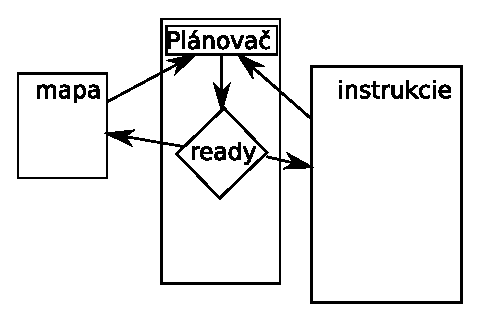
\includegraphics{planovac.eps}
\caption{ Práca plánovača }
\label{fig::planovac}
\end{figure}
Robot by mal vykonávať svoj algorimus dovtedy, pokiaľ ho niekto externe nezničí. To znamená, že algoritmus sa musí opakovane vykonávať potenciálne do nekonečna. No nie je vhodné, aby na to dával pozor sám hráč, Jednak by to musel opakovane deklarovať u každého svojho naprogramovaného robota a jednak táto deklarácia je iba manuálny zapis, ktorý nemá vplyv na použitú stratégiu. Preto sa v práci dbá na to, aby v okamihu, keď by mal robot skončiť  jeho algoritmus, spustil odznova v nekonečnom cykle.% prej nezrozumitelne

%penalizáacie ... juchuuuuuuu<<< suhlas
Doteraz sme mlčky predpokladali, že každá časť algoritmu má rovnakú váhu. Tým, že niektoré časti algoritmu vyhlásime za ťažšie spraviteľné, potom vytvoríme novú inštanciu sveta. Tam sa nemení obsah, ale spôsob narábania s algoritmom. Hráč potom musí vymyslieť taký algoritmus, ktorý počíta s daným nastavením. \\
Potrebujeme ale vedieť, že to skutočne prispeje k atraktívnosti hľadania vhodnej stratégie. Rozoberme si teda, ako to bude vplývat na algoritmus, ak by jednotlivé časti trvali iný počet kôl. Potom by bol užívateľ nútený použiť taký algorimus, ktorý dlho trvajúce časti použiva minimálne. Napriklad, ak by robotovi trvalo štyri kola na to, aby sa otočil, potom hráč sa pravdepodobne bude snažiť použiť minimálny počet otočení.
Tým spôsobom sa môže vymýšlanie stratégií posunúť na hlbšiu úroveň, čo vyhovuje nároku na prácu.\\%ako je ukazane na obrazku:<<< rad sa kuknem
Výsledne plánovače potom dostanú iné vlastnosti. %mozno obrazok?
\subsection{Možné prístupy k programovaniu virtuálneho sveta}
Dôležitou časťou práce je predstaviť spôsob, akým bude užívateľ zapisovať vymyslený algoritmus. Uvažujeme nasledujúce jazyky: %<<< Hmmm, najdolezitejsej casti bude dalsia kapitolka?bude, bude
\begin{description}
\item [Grafický jazyk] \hfill \newline
Pod grafickým jazykom rozumieme jednoduché grafické zobrazenie zápisu algoritmov. Tento spôsob sa najskôr využival pri výuke programovacich jazykov ako ľahký a zrozumiteľný spôsob písania algoritmu. Jednoduchým sledovaním šipiek v zápise sa dá zistiť, v akom stave sa program nachádza pri počiatočnych podmienkách. %proste budeme iba sledovat sipky
%jak to funguje, ked je to grafické. ( prehľadne a cool )
Implementovanie vlastného grafického jazyka, kde by boli príkazy len pre potrebu programátora, by bola dosť náročná. Jediný nástroj, ktorý splňoval základné predstavy, bol ale Microsoft Visual Language\cite{msvl}, ktorý je pre nekomerčné využitie síce zdarma, bohužiaľ je závislý na operačnom systéme, takže sa ukázal ako nevhodný \\ 
\item [scriptovací jazyk LUA]\hfill \newline
LUA\cite{lua} je scriptovací jazyk, ktorý sa využíva práve na programovanie problémov umelej inteligencie, čo je aj náš prípad. Jeho výhodou je, že tento jazyk je jednoduchý, voľne širiteľný a prenositeľný. \\
LUA je však konštruovaná tak, že kompletne prevedie daný algoritmu, takže by sme nemali priamu kontrolu nad jednotlivými časťami kódu. Napríklad kontrola obsadeného úložisťa, ktoré môže robot použivať, by sa skomplikovala. Rovnako rozhodnutie, kedy algoritmus vykonal dosť príkazov a je nutne ho pozastaviť. Preto nebol použitý jazyk LUA.
%\item [XML] % to sa este rozmyslim
\item [Vlastný jazyk]\hfill \newline
Ďalšou možnosťou je vytvoriť vlastný jednorázový Domain Specific Language, ktorý bude použiteľný len na úlohy typu Codewars. Ponúka kompletný dohľad nad kódom, rozhodli sme sa preto pre tento koncept.
\item[Vyšší programovací jazyk]\hfill \newline
%TODO
\end{description} %snad to staci, je to kratke, ale co uz, spisovatelka zo mna nebude<<<to nie je take iste - ani ja som nechcel byt pedagogom.;)
\subsection{Robotština}
Algoritmus bude teda zapísaný vo vlastnom jazyku - robotštine. To naň kladie netriviálne nároky.
\subsubsection{Minimálne schopnosti}
Na začiatku je dôležité vedieť, čo všetko by mal jazyk ponúkať, aby sa pomocou neho dal napísať plnohodnotný algoritmus chovania robota v popísanom svete. \\
Robot musí pomocou popísaného algoritmu ovládať akcie, ktoré smie robiť, aby vôbec vo svete niečo vykonal. Jazyk preto bude obsahovať príkazy na 
\begin{itemize}
\item pohyb 
\item čakanie (ako opak pohybu - ničnerobenie na istý počet kôl)
\item útok
\item otočenie sa
\item získavanie informácií o objektoch z okolia - viditeľnosť
\end{itemize} % to je vsetko, co moze robot vizualne robo
Tieto príkazy podmieňujú vznik operacií s objektami.
%POZOR tu to pisem zmatene, mi pride, ze idem do hlbky a asi by som mala do sirky
\begin{description}
\item[Pohyb] znamená, že robot sa pohne daným smerom niekoľko krokov. Počet krokov je intuitívne vyjadrený celým číslom. V okamihu vykonávania príkazu nemusíme ešte presne vedieť, o koľko krokov sa robot pohne, preto je potrebné zaviesť premenné.
\item[Premenné] v zmysle ich  definície uchovávajú určité informácie. Vzhľadom na náš virtuálny svet potrebujeme, aby uchovavali: %nebola by lepsia tabulka?
\begin {itemize}
\item celé číslo - {\it Integer}
\item reálne čislo -- spresnenie celého čísla kvôli aritmetickým operáciam, ako je ďalej uvedené - {\it real}
\item objekt sveta {\it Object}
\item pozíicia sveta ako dvojrozmerný vektor {\it Location}
\item pole premenných - {\it int[3], real[a][3], location[4] } %toto nechcem okecat, snad je to z  toho jasne<<<staci
\item {\it null} pre oznámenie robotovi, že nemá uložený žiadny objekt
\item {\it this} pre referenciu svojho vlastneho objektu
\end{itemize}  
%mozno, co je este nepotrebne, ale to podla mna netrena, hovorim o tom, co tam nezpodmienecne musi byt
\item[Operácie s číslami] sa objavujú v súvislosti s premennými. Budú podporované iba niektoré základné operácie s reálnymi čislami, a to :
\begin{itemize}
\item sčítanie
\item odčítanie
\item násobenie
\item delenie, pričom výsledok delenia celých čisel bude reálne číslo
\item zvyšok po delení pre celé čisla = {\it \%}
\end{itemize}
Ostatné aritmetické operácie nebudú podporované, nakoľko nie sú nevyhnutne potrebné. Aby sme docielili výsledok delenia v celom čisle, reálne a celé čísla sa navzájom automaticky konvertujú. Uživateľ toto nemusí špeciálne ošetrovať. %>>>kedze jazyk nema simulovat matlab. %;) Chcem povedat, ze MNE to staci, ostatne sa z toho daju spravit
\item [Operácie s objektami] dávajú možnosť reagovat na svet,  t.j. umožňujú zistiť:
\begin{itemize}
\item akým smerom je objekt otočený (vhodné pre robota, aby zistil, či nie je na muške ) {\it getDirection (o) }
\item akým smerom sa objekt pohybuje { \it isMoving(o) }
\item či je to strela, stena alebo robot -{\it isMissile(m), isWall(o), isPlayer(p), isEnemy(o) }
\item či bol nepriateľský robot zasiahnutý - {\it isHit(robot)}
\end{itemize}
\item[Relačne operácie] $>, <, =, \ne $ a ich kombinácia pre všetky typy premenných. Využijú sa napríklad pri zisťovaní najbližšieho objektu, atd. Pre objekty je nezmysel porovnavať, či je menší alebo väčši, preto u objektov je povolený iba relačný operátor $=$ a $\ne$.
\item[Podmienky] výrazne prispievajú k eliminovaniu  pre robot nepríjemných udalostí, ktoré môžu vo virtuálnom svete nastať (ak je tam mína, tak tam nesľapni). Viažu sa k nim ďalšie kódové slová TRUE (1) a FALSE (0).
\item[Cykly] zjednodušujú prácu pri vykonávaní rovnakých časti kódu. Podporované sú cykly s podmienkou na začiatku, na konci, pevný počet opakovaní a počet opakovaní v závislosti na premennej, s ktorou sa dá manipulovať. % je to ok (while a tak?)ano, presne tak, je to dobre vyjadrenie?
\item[Procedry a funkcie] umožňujú sprehľadňovať a členiť kód. Prispievajú k lepšiemu kódovaniu algoritmov, využívaniu pamäte, ktorá sa po skončení procedúry uvoľní. Parametre k funkciám sa dajú predávať odkazom alebo referenciou.  Definovanie predávania parametra referenciou je značené kódovým slovom {\it ref} pred premennou, ktorá je takto predávana. Poradie parametrov predávaných odkazom a hodnotou nehrá rolu. Parameter s preddefinovannou hodnotou nie je podporovaný %a to NEMIENIM zdovodnovat
\item [Definovanie cieľov a vlastností] reprezentuje chovanie robotov. % <<< viac netreba %tu uz neviem, co mam napisat
\end{description}

Premenné sa ukladajú do úložiska. Ak už nie je voľné miesto v pamäti, bolo by nemilé, aby robot umrel. Rovnako je to nefér aj voči robotom, ktorý ho lovia. Namiesto toho bude premenná ukazovať na miesto v pamäti, ktorá je už obsadené. Robot tak pri nešetrnom zachádzaní s pamäťou môže poškodiť sám seba na úrovni programu, čo zahŕňa princíp škodenia, aký je v Aresovi.
%mysleno prepise uz existujucu premennu, ktora tam uz je
Algoritmus môže efektívne prepísat hodnotu, na ktorú sa spolieha, ale to zodpovedá tomu, že sa robot z nedostatku úložišťa zbláznil. Obzvlásť  je to viditeľné, ak si prepísal premennú, na ktorú sa spolieha. Napríklad hodnotu TRUE bude zrazu FALSE. \\

Aby sa predišlo týmto nepríjemnostiam, je vhodné vedieť, kedy premenné vznikajú (v zmysle obsadzujú pamať) a kedy zanikajú (uvoľnujú pamät). \\
Pri deklarovaní premennej sa táto automaticky vytvorí, čo je normálne chovanie, známe takmer vo všetkých vyšších programovacích jazykoch. Pri volaní funkcie s parametrami sú tieto parametre kopírované, pokiaľ neboli definované kódovým slovom ref. To znamená, že sa vytvoria znova všetky premenné a pridá sa im hodnota, s akým je funkcia volaná. Návratova hodnota sa vytvorí v okamžiku volania {\it return}. V prípade, že ide o procedúru, návratová hodnota sa nevytvorí.
Premenná sa môže dočasne vytvoriť aj v bloku označenom \{\}. Po ukončení bloku sa premenná v úložisku uvoľní. Preto by sa v nasledujúcom kóde (mimo bloku) mohla dať použiť. Premennú s rovnakým menom nie možné vzhľadom na implenentáciu vytvoriť ďalej s iným typom, než bola prvýkrát deklarovaná. Toto ale nie je závažný problém, keďže sa jedná iba o vytvorenie názvu pre premennú a rovnaké mená s rôznym typom iba mätú neskoršieho čitateľa. \\

Premenná obsadzuje miesto v úložisku. Vzhľadom na obmedzenie úložiska je namieste určiť, aké množstvo jednotiek úložiska jednotlivé premenné zaberajú. Premenné typu Object, Real a Integer budú zaberať jednu jednotku miesta, pretože nemá ďalej zmysel deliť ich na menšie časti. V reálnych jazykoch tomu tak pochopiteľne nie je, tu sme to obmedzili preto, aby obsadzovanie pamäte bolo jednoduché a pochopiteľné. Ďalej je u je typ Location. Ten má z princípu dve zložky. Preto v pamäti bude zaberat 3 jednotky, pre 3 premenné typu integer, ktoré sú jej zložkami a jednu pre seba. Podobne obsadzujú pamäť zložné prvky (polia). To znamená jedno pre samotnú premennú a potom súčet obsadenia všetkých jeho premenných. \\%snad je to tu jasne

\subsubsection{Syntax robotštiny}
Algoritmus je možné zapísať pomocou sekvencií príkazov. Pre správne pochopenie algoritmu je nutné definovať ich gramatiku. Tú zobrazuje obrazok <OBR-TODO>
kde :
\begin{description}
\item [vlastnosť] je jedno z:
\begin{itemize}
\item hipoints (počet životov)
\item attack ( veľkosť útoku )
\item mAttack ( veľkosť útoku strely )
\item mHealth ( dostrel/životnosť strely )
\item angle ( veľkosť uhla viditeľnosti )
\end{itemize}
nasledované číslom, ktoré definuje vlastnosť. V prípade, ak užívateľ počet bodov prekročí alebo podcení, vlastnosti sa budu škálovať.
\item [Ciele algoritmu] sa skladajú z:
\begin{itemize}
\item $visit | visitSequence ( [X,Y] | X )$
\item $kill [a-zA-Z0-9]*$
\item $killed <|>|<=|==|!=|>=$
\end{itemize}
\item [Príkaz na robota] je príkaz z množiny $step(X), wait(X), see(), eye(X), turn(X) X\in N, seeEnemy()$
\item [Príkaz na informáciu] je príkaz z množiny $(Locate(o), isWall(o), is Player(o), isEnemy o \in Objekt, seen[n] n\in N  $ %kontrola, ci je tu vsetko
\end{description}
\subsubsection{Príklady použitia} %snad nemusia robit nic konkretne
Nasledujúce príklady vysvetľujú, ako sa použivajú jednotlivé príkazy, nemajú však za úlohu demonstrovať skutočný kód
\begin{verbatim}
robot R1 {
    attack = 20
    mAttack = 100
    hitpoint = 60
    memory  =10
    kill R2
    killed ! = 1 
    integer l = 10;
    main()
    {
    	for (integer i = 0; i < l; i++)
        {
            while (see()>0 && isPlayer[seen[0]])
                shoot(seen[0]);
            turn (30);
        }
    }
}
robot R2 {
    target ( Start[ R1 ], Start [R2])
    kill < 2
    Location was = [0,0]
    main()
    {
        Location l = [-1,-1];
        turn (getTarget());
        while (step(4) != 0)
        {
            if (was == l)
            {
                turn(15);
                continue;
                was = locate(this);
            }
            turn ( -direction(l));
        }        
    }
\end{verbatim}
%STUDIUM príkazov je nad moje schopnosti, no vyzeraju doveryhodne

